\chapter{Experimental Protocol and Results}\label{ch:protocol}
The completed protocol is pipeline-oriented. Configuration records seed, input size, padding color, model names, normalization, split sizes, retrieval gallery, top-$k$, and query count. The image preprocessing comparison evaluates letterbox, stretch, and center crop on the existing 100 validation images using geometric criteria only. Letterboxing preserves the entire image and aspect ratio, at the cost of padding. Mean content fraction is 0.7224 and padding fraction 0.2776; stretch has mean absolute log aspect distortion 0.3309; center crop discards a mean 0.2776 of image area. This is a new geometry-based comparison, not a historical model-performance experiment.

For retrieval smoke testing, 20 evenly spaced validation/test image embeddings query the 10,000-image training gallery. The evaluator requests top five and removes any same-ID match. Caption index construction separately checks source ordering, unique training caption IDs, and zero held-out caption IDs in the knowledge base; a self-query smoke check excludes the source vector when selecting a neighbor. No generation prompts, decoding parameters, human evaluation, or caption metric computations are present.

The geometric comparison visualization is included in \cref{fig:preprocess}; it visualizes the same criteria and summary values in \cref{tab:preprocess}. The selection favors full field-of-view and aspect preservation, not measured captioning performance.

\begin{table}[htbp]\centering\caption{Preprocessing comparison on 100 validation images.}\label{tab:preprocess}
\small\begin{tabularx}{\textwidth}{lXXXX}\toprule Configuration & Content fraction & Aspect distortion & Crop fraction & Padding fraction\\\midrule Letterbox 224 & 0.7224 & 0.0000 & 0.0000 & 0.2776\\Stretch 224 & 1.0000 & 0.3309 & 0.0000 & 0.0000\\Center crop 224 & 0.7224 & 0.0000 & 0.2776 & 0.0000\\\bottomrule\end{tabularx}\end{table}
\begin{figure}[htbp]\centering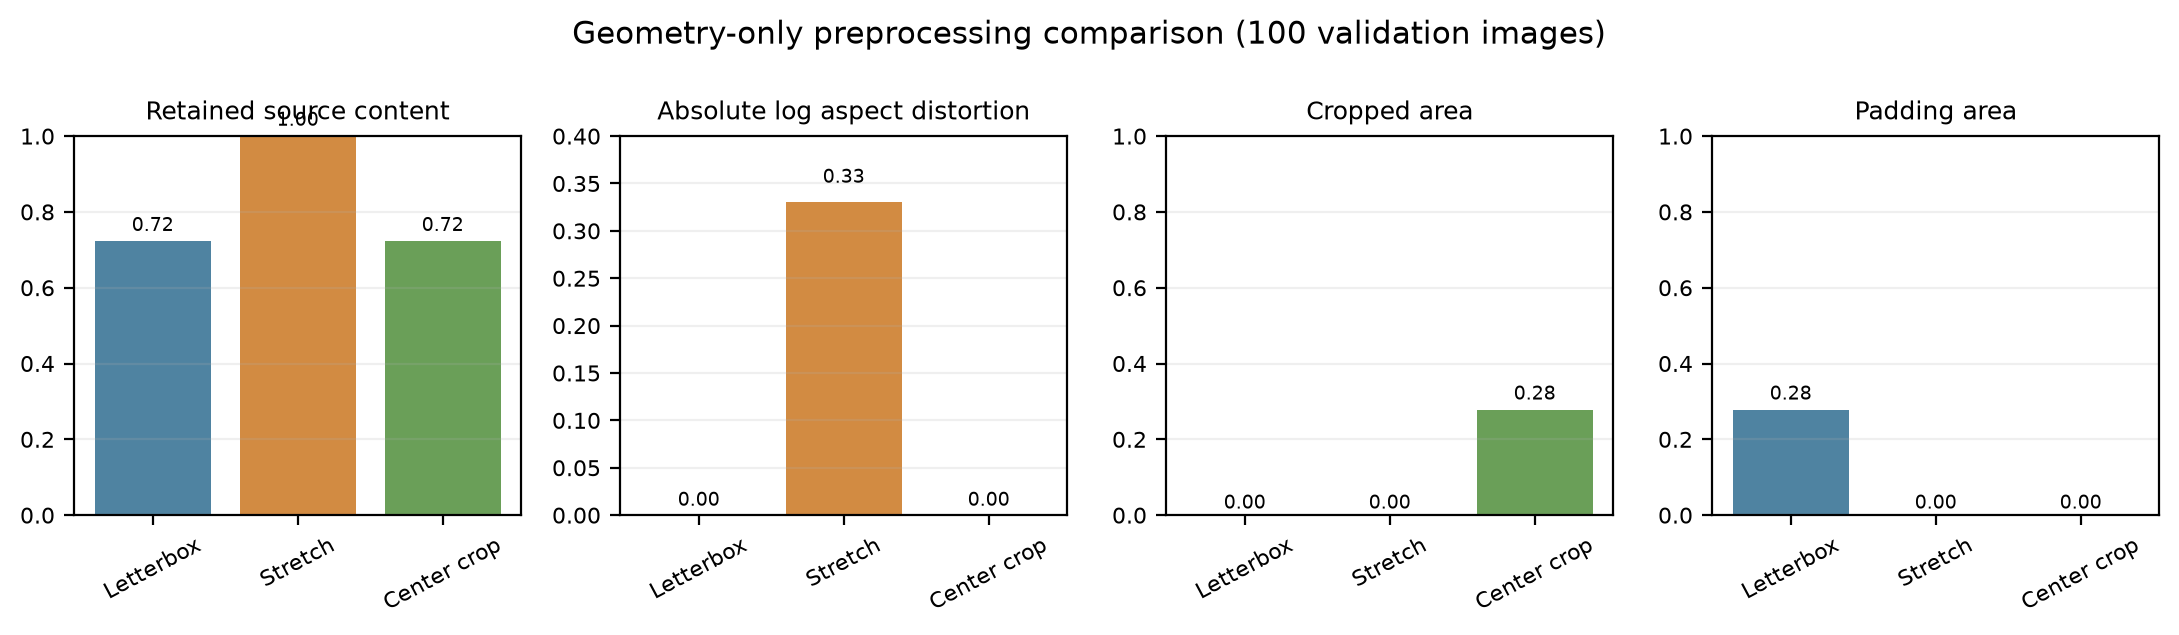
\includegraphics[width=0.94\textwidth]{preprocessing_geometry_summary.png}\caption{Geometry comparison on 100 validation images; no downstream model performance was measured.}\label{fig:preprocess}\end{figure}

\section{Quantitative Results}\label{ch:results}
The quality-control report records PASS for all applicable Phase 1 checks, with zero failed, warning, or not-run checks. It verifies 10,000/100/1,000 image records, corresponding 50,000/500/5,000 captions, complete image decoding, split disjointness, exact and perceptual hash checks, vector shapes/norms, mapping order, and FAISS readback. The summary is shown in \cref{tab:qc}. The report's PASS describes the checks implemented by the repository; it must not be read as full project or assignment completion.

\begin{table}[htbp]\centering\caption{Selected quality-control outcomes recorded by the project.}\label{tab:qc}
\begin{tabularx}{\textwidth}{lX}\toprule Check & Recorded result\\\midrule Processed-image decode & 11,100 decoded; 0 errors; 0 missing files\\Split overlap & 0 pairwise overlaps\\Exact duplicate check & 0 SHA-256 duplicate groups\\Perceptual duplicate audit & 11,100 hashed; 9 within-split candidates; 0 cross-split candidates at threshold 6\\Image embedding integrity & Train 10,000; validation 100; test 1,000; 512-D, finite, unit norm\\Caption embedding integrity & 50,000 train vectors; source order valid; held-out caption IDs: 0\\Index readback & Image 10,000 and caption 50,000; dimension 512; valid\\\bottomrule\end{tabularx}\end{table}

Image retrieval returned results for all 20 held-out queries, each with five neighbors, and no self-matches. The complete summary is in \cref{tab:retrieval}. Mean top-1 cosine similarity was 0.8260029644. The value measures similarity between CLIP image embeddings and training gallery items; without relevance judgments it does not quantify retrieval precision or caption quality. The caption index smoke test returned a nearest non-self caption with cosine 0.9504 for its first training caption query; this is a single construction check, not an aggregate evaluation.

\begin{table}[htbp]\centering\caption{Held-out image retrieval smoke test.}\label{tab:retrieval}
\begin{tabular}{lr}\toprule Measure & Value\\\midrule Queries & 20 (validation/test)\\Gallery & 10,000 train images\\Requested neighbors & 5\\Successful query results & 20/20\\Self matches & 0\\Mean top-1 cosine similarity & 0.8260\\Index readback & Valid\\\bottomrule\end{tabular}\end{table}

\section{Dataset Exploration}\label{ch:exploration}
\section{Object categories and scene complexity}
The train2017 annotation audit covers 80 object categories. Person instances account for 262,465 of 860,001 instances (30.52\%), followed by cars (43,867; 5.10\%) and chairs (38,491; 4.48\%). The distribution is long-tailed, as illustrated by the repository's top-50 frequency visualization (\cref{fig:cats}). Instance counts have mean 7.27 and median 4 in the complete train2017 annotation pool; counts range from zero to 93. Selected image complexity labels are based on source-pool quartiles of nonzero object count (Q1=2, Q3=10), not a learned scene-complexity model.

\begin{figure}[htbp]\centering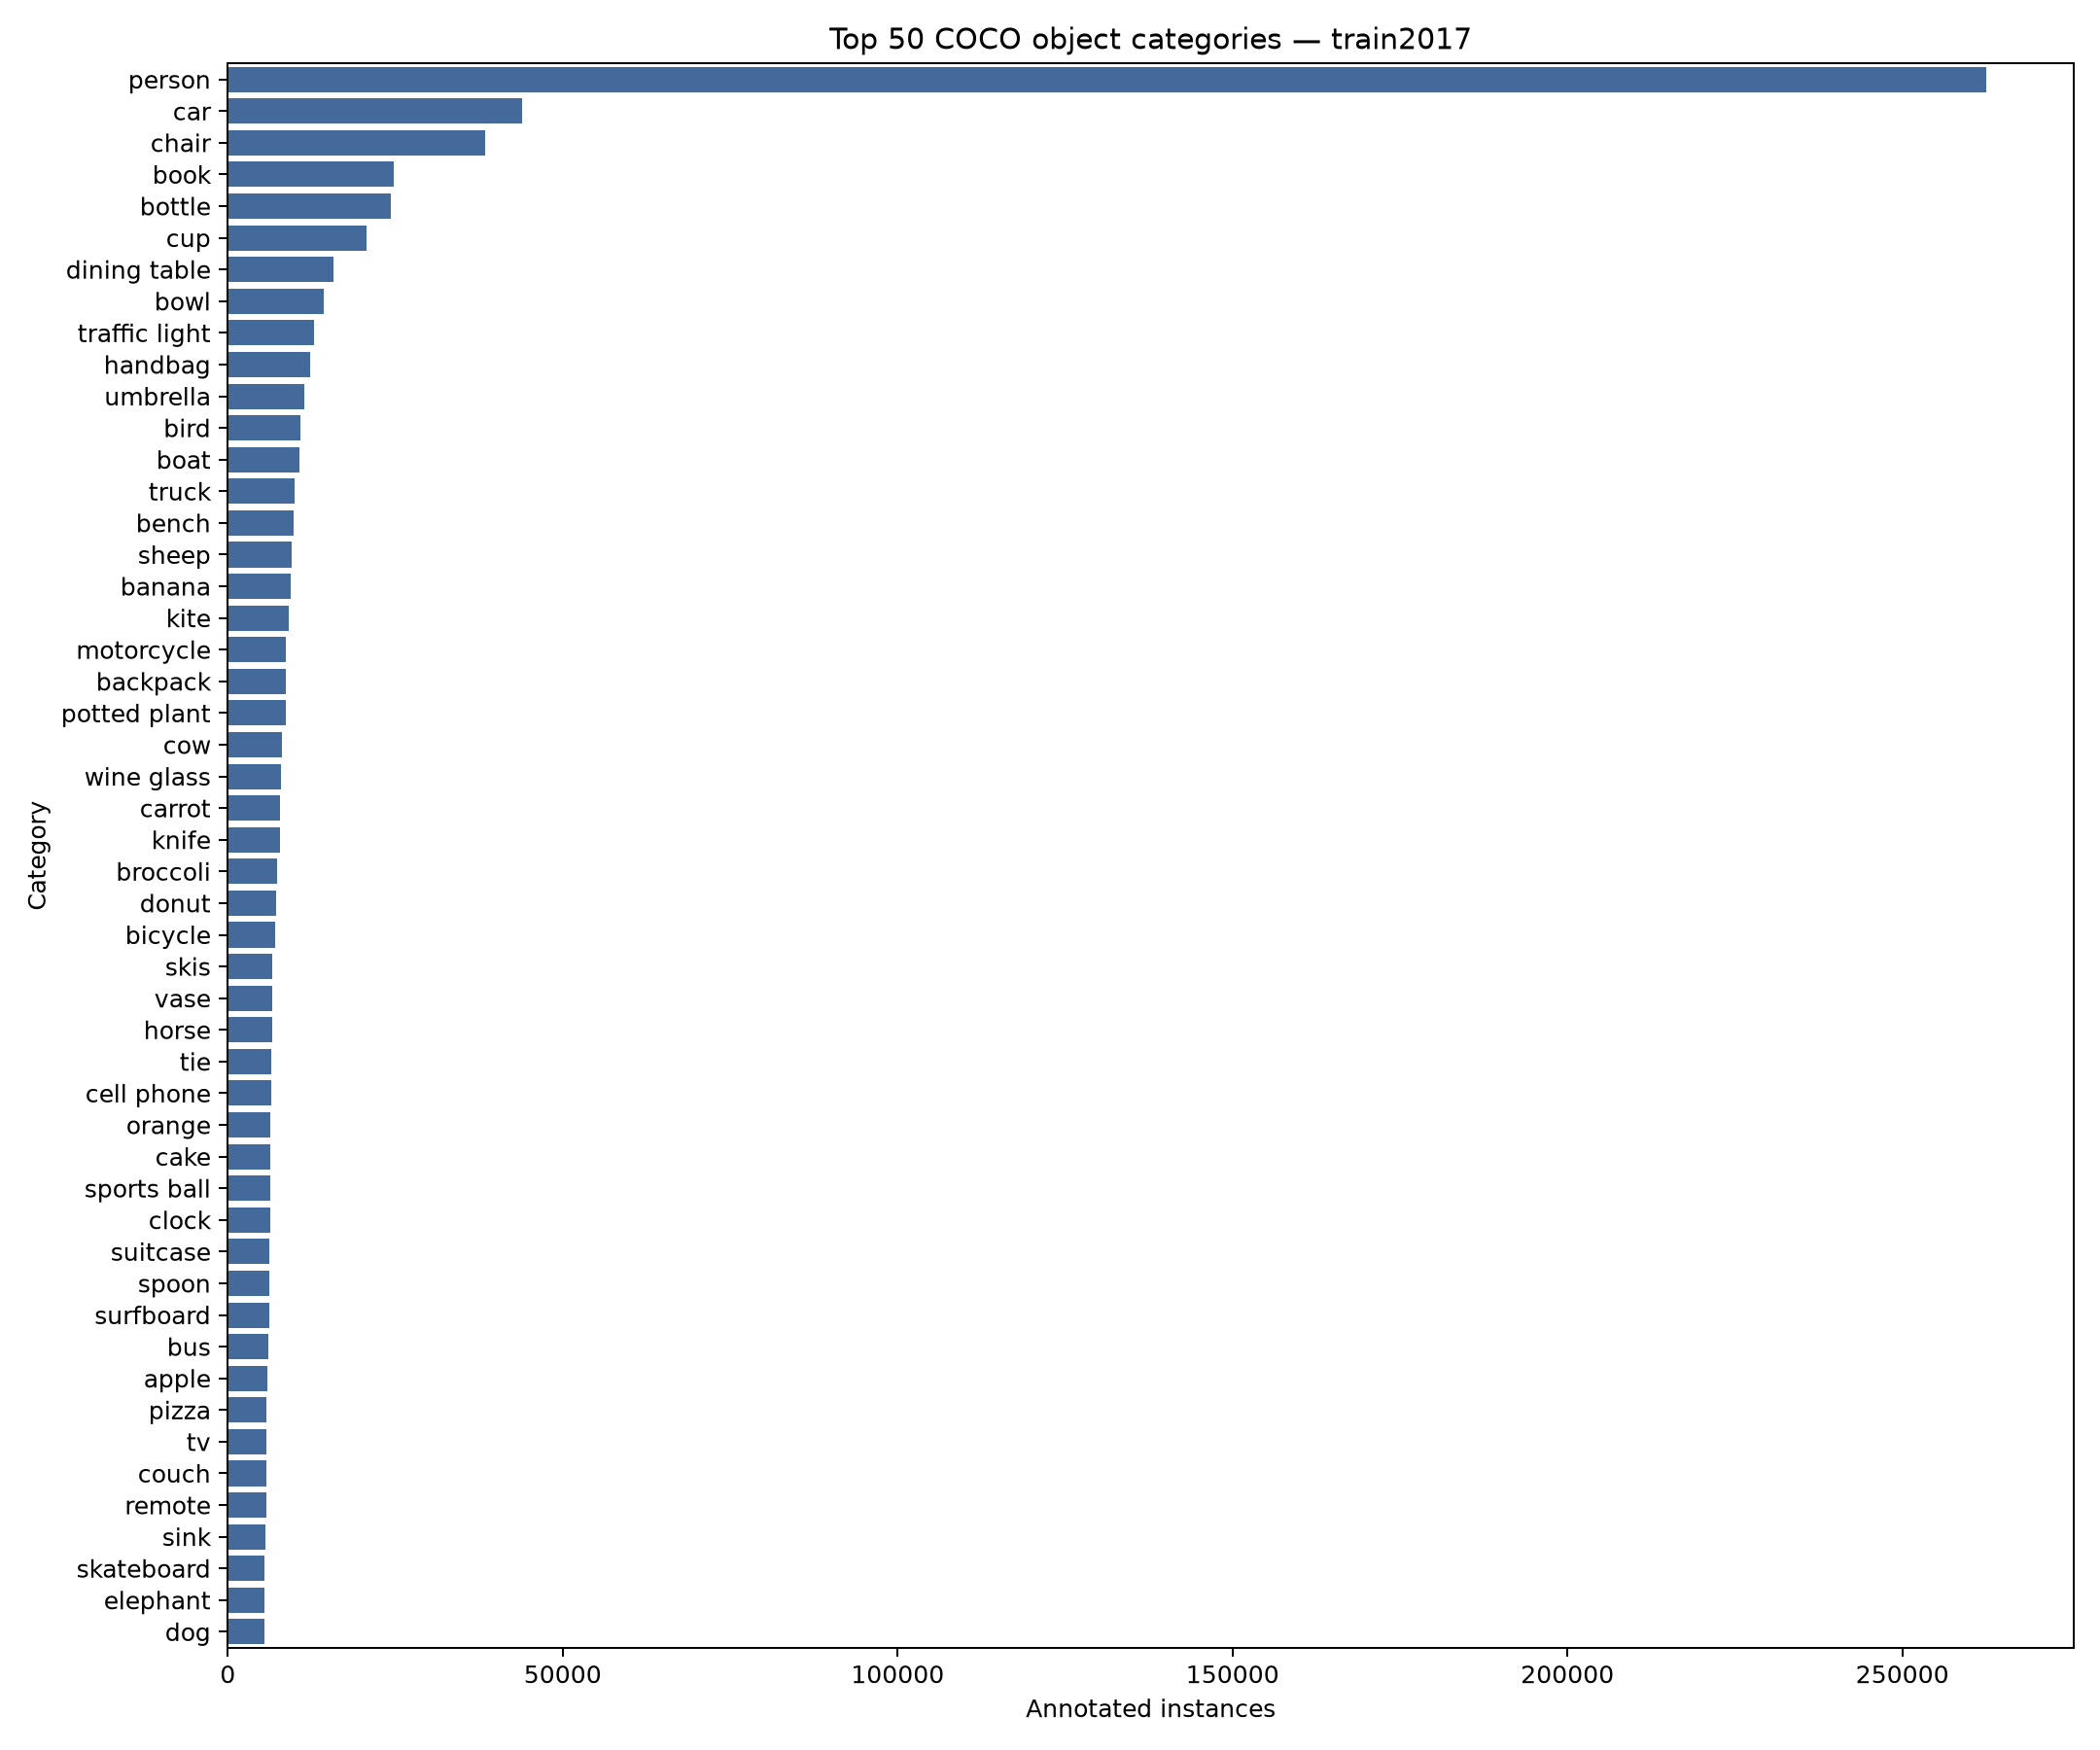
\includegraphics[width=0.88\textwidth]{top50_object_classes.png}\caption{Frequencies of the 50 most common COCO object categories in train2017 annotations. Annotation counts are not caption-generation results.}\label{fig:cats}\end{figure}

\section{Captions and vocabulary}
Every selected image has five references. A Unicode NFKC-normalized, case-folded tokenizer recognizes Unicode letters and numbers and retains internal apostrophes; it does not stem or lemmatize. Across all 55,500 references, the extended analysis reports 591,664 tokens and 9,793 unique tokens. A distinct spaCy POS stage covers 55,500 captions, records 642,147 model-tokenized tokens, and reports zero processing errors. The token totals differ because the analyses use different tokenization systems and definitions. They should not be conflated. Caption length, word frequency, and vocabulary-rank charts are available in the repository; example length and POS distributions are shown in \cref{fig:captions,fig:pos}.

\begin{figure}[htbp]\centering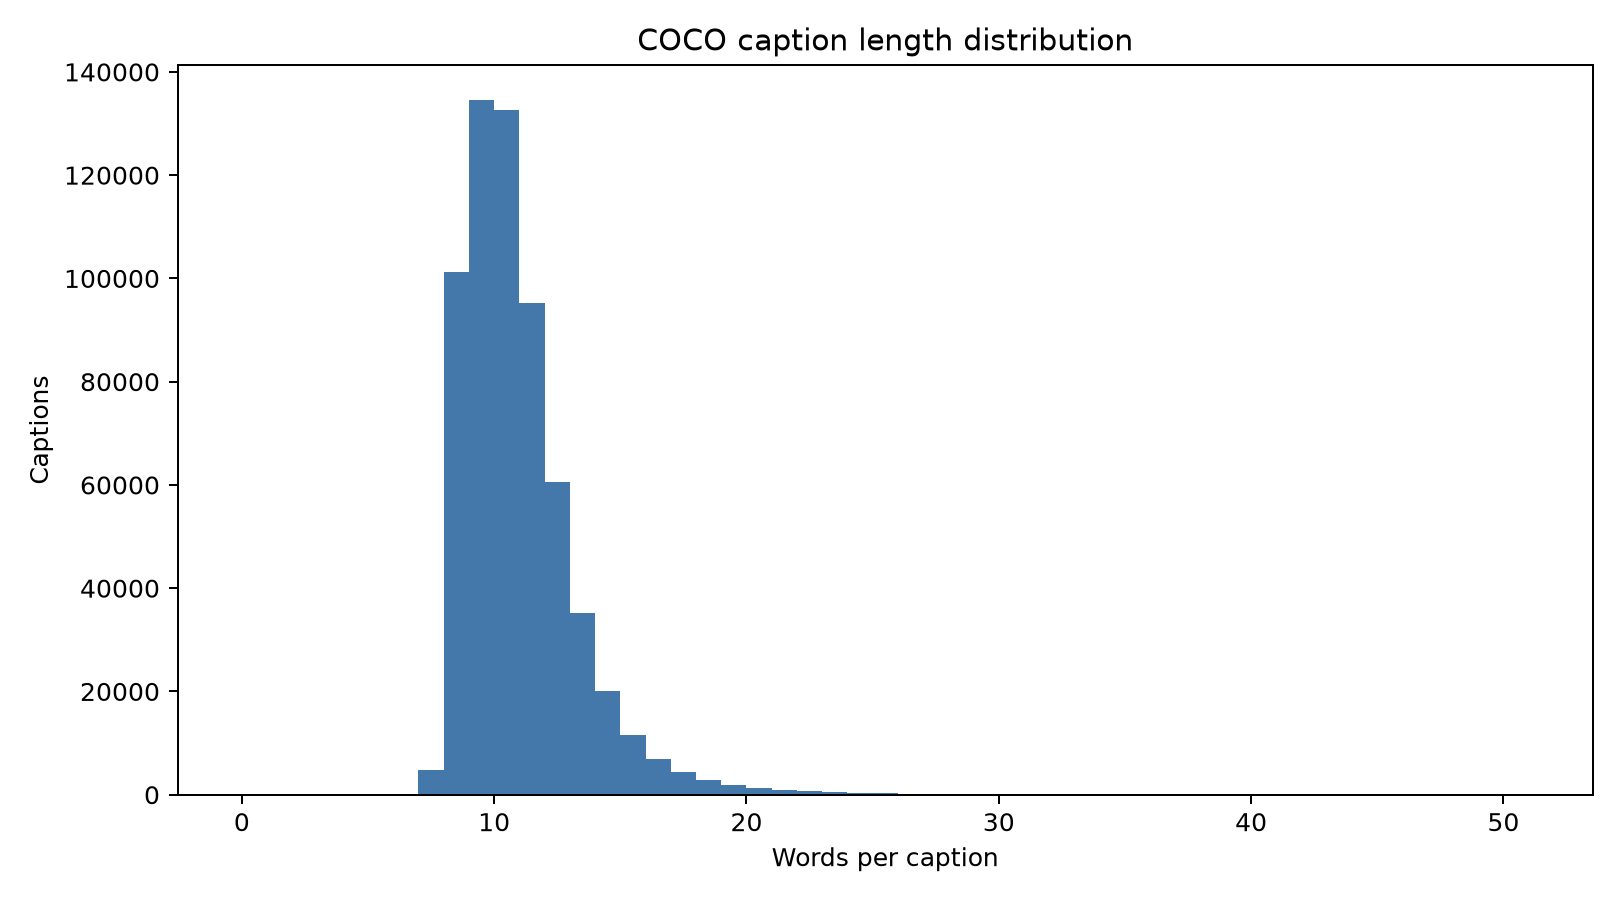
\includegraphics[width=0.8\textwidth]{caption_length_distribution.png}\caption{Caption-length distribution generated by the project caption analysis.}\label{fig:captions}\end{figure}
\begin{figure}[htbp]\centering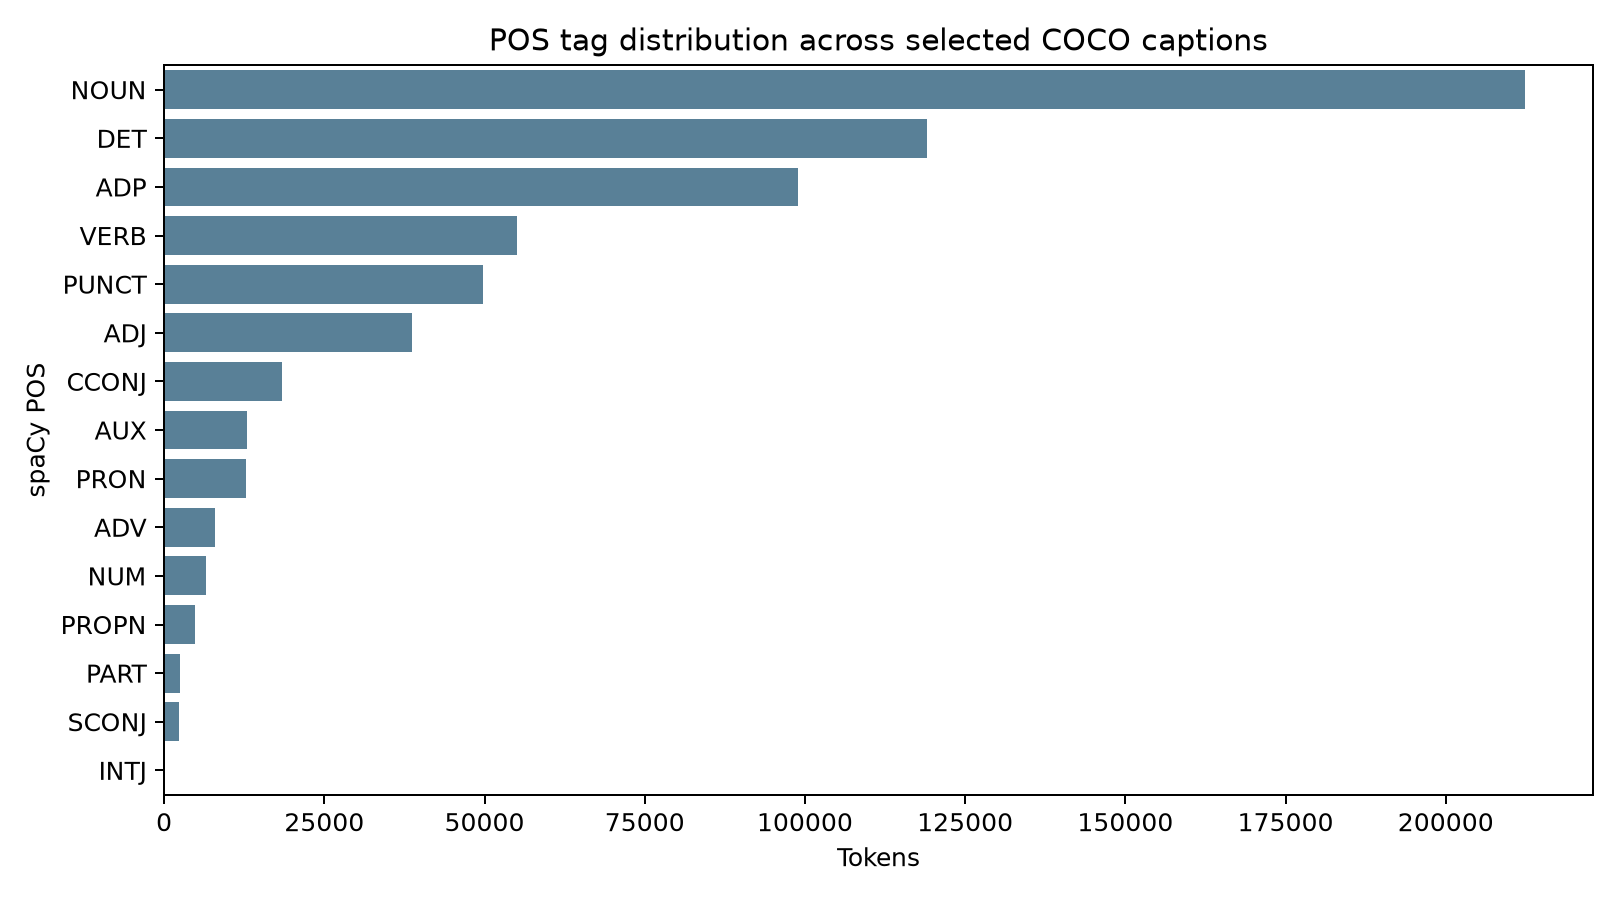
\includegraphics[width=0.8\textwidth]{caption_pos_distribution.png}\caption{spaCy part-of-speech token distribution across selected captions; tags are model predictions.}\label{fig:pos}\end{figure}

\section{Bounding-box geometry}
The project computes pairwise box relations from COCO instance boxes. It counts centroid ordering (left/right and above/below), containment, intersection-over-union overlap (IoU at least 0.10), and proximity by normalized center distance at most 0.10. Across 11,100 selected images the recorded pair counts include 680,482 left-of, 671,396 below, 676,706 right-of, 584,569 above, 47,381 overlapping, 151,587 near, 28,366 contains, and 30,359 inside. These are calculations over annotated object boxes, not COCO semantic relationship labels. They do not prove interaction, contact, support, or action. The relationship chart is presented as descriptive geometry only (\cref{fig:relations}).
\begin{figure}[htbp]\centering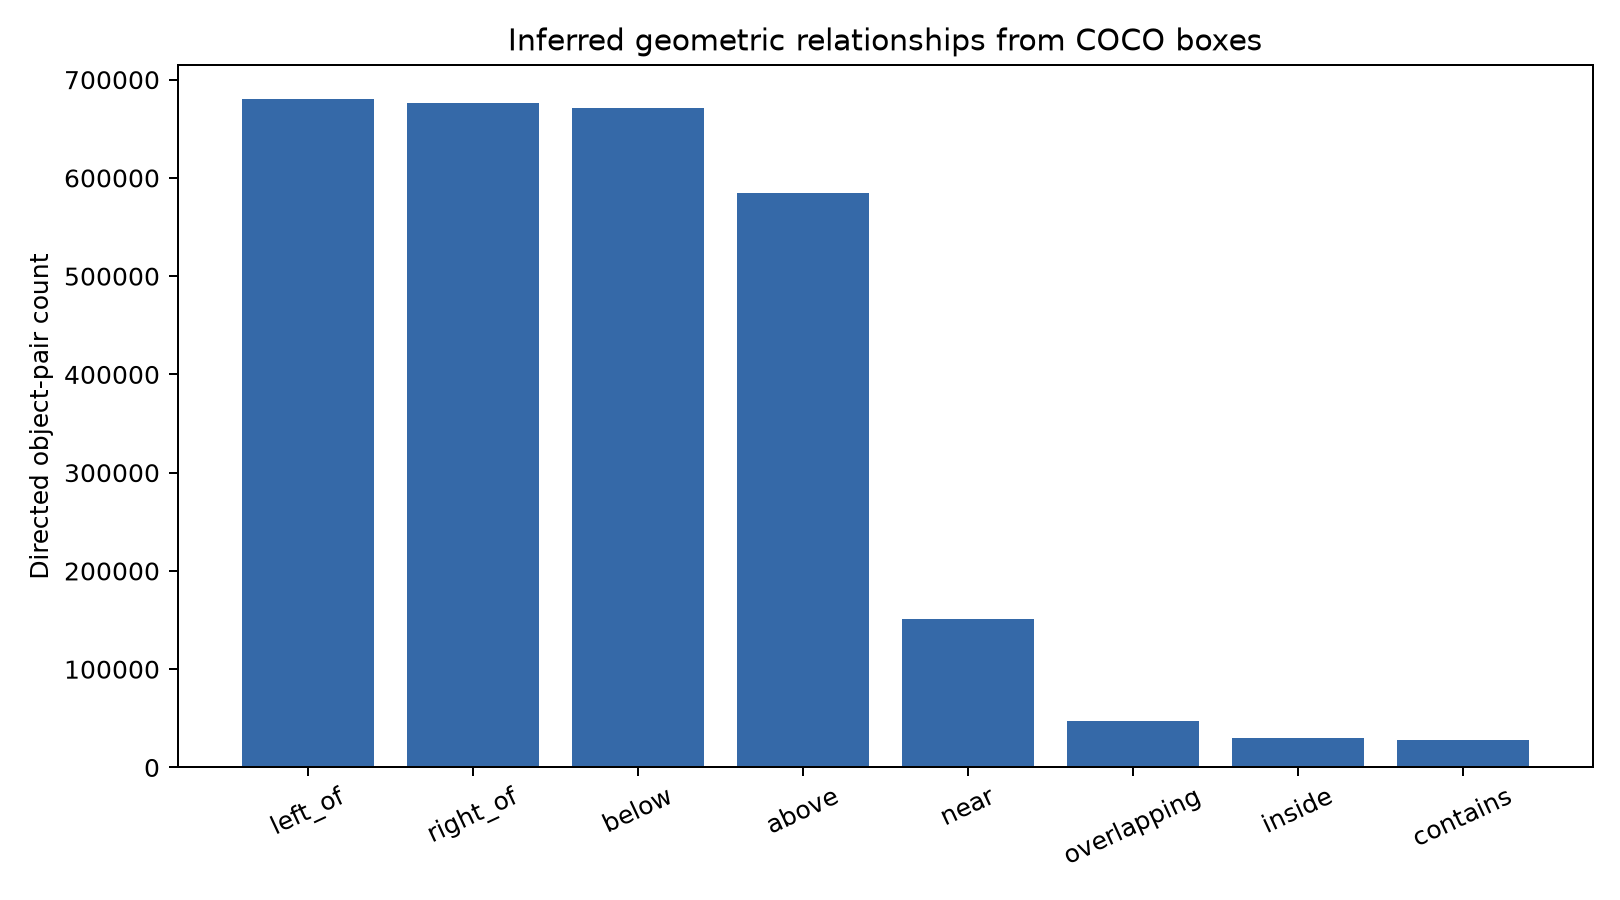
\includegraphics[width=0.88\textwidth]{geometric_relationship_frequencies.png}\caption{Counts of box-derived geometric relationships in selected images. Relation terms are operational geometric rules, not semantic ground truth.}\label{fig:relations}\end{figure}

\section{Pixel-level visual analysis}
The color analysis samples image pixels and maps hues to coarse color families; luminance and saturation summaries are image-level measures. Its dominant-color counts include red 4,430 and gray 3,948 images, with the remaining image counts spread among other color families. The method does not identify the color of a particular object. A global edge-density proxy uses image edges and is not object segmentation or shape recognition. Scene/context/day-night tags are zero-shot CLIP prompt predictions with confidence thresholds and abstention; their softmax scores are relative and uncalibrated. These sources are kept separate from COCO annotation labels. See \cref{fig:color,fig:scene}.
\begin{figure}[htbp]\centering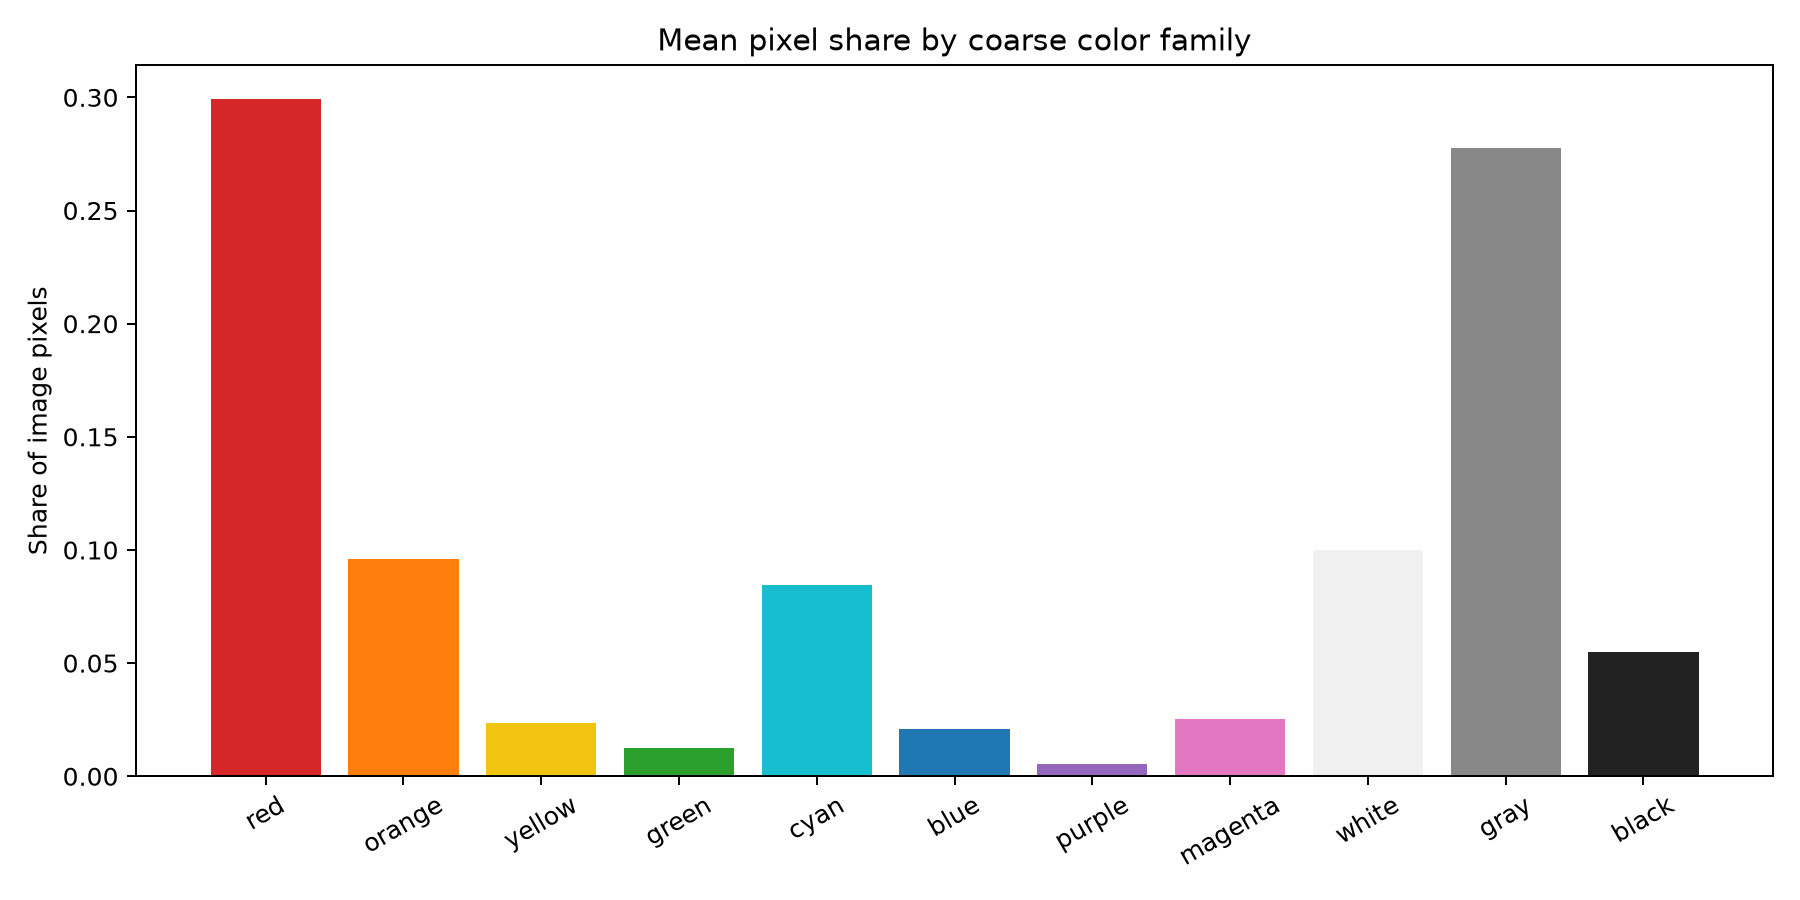
\includegraphics[width=0.78\textwidth]{color_family_distribution.png}\caption{Coarse dominant pixel-level color-family analysis over the selected images.}\label{fig:color}\end{figure}
\begin{figure}[htbp]\centering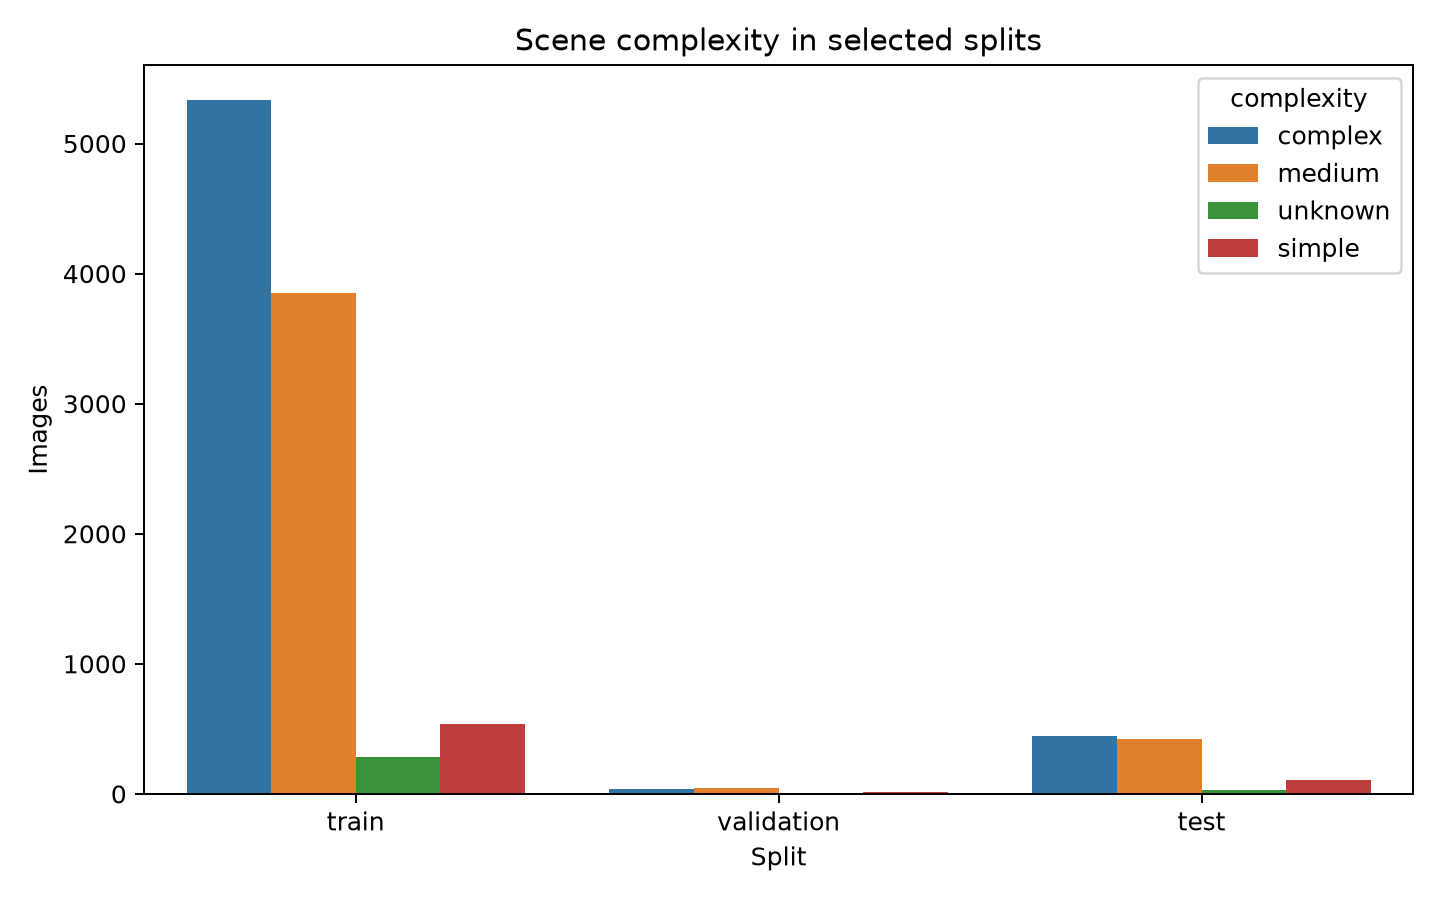
\includegraphics[width=0.78\textwidth]{selected_scene_complexity.png}\caption{Selected-image scene-complexity distribution based on annotation counts.}\label{fig:scene}\end{figure}
